\pdfoutput=1

%\documentclass[preprint,10pt]{elsarticle}
%\documentclass[preprint,10pt]{amsart}
\documentclass[review]{siamart0216}
%\documentclass{siamart0216}

%\usepackage{fullpage}
%\usepackage[colorlinks=true]{hyperref}

\usepackage{amsmath,amssymb,amsfonts}
%\usepackage{amsthm}
%\theoremstyle{definition}
%\newtheorem{definition}{Definition}
%\theoremstyle{lemma}
%\newtheorem{lemma}{Lemma}
%\theoremstyle{corollary}
%\newtheorem{corollary}{Corollary}
\newtheorem*{remark}{Remark}
%\theoremstyle{theorem}
%\newtheorem{theorem}{Theorem}
%\theoremstyle{assumption}
%\newtheorem{assumption}{Assumption}

\usepackage[titletoc,toc,title]{appendix}

\usepackage{array} 
\usepackage{listings}
\usepackage{mathtools}
\usepackage{pdfpages}
\usepackage[textsize=footnotesize,color=green]{todonotes}
\usepackage{bm}
\usepackage{bbm}

\usepackage{tikz}
\usepackage[normalem]{ulem}
\usepackage{hhline}

\usepackage{graphicx}
\usepackage{subfig}
\usepackage{color}

%% ====================================== graphics

\usepackage{pgfplots}
\usepackage{pgfplotstable}
\definecolor{markercolor}{RGB}{124.9, 255, 160.65}
\pgfplotsset{
compat=1.3,
width=10cm,
tick label style={font=\small},
label style={font=\small},
legend style={font=\small}
}

\usetikzlibrary{calc}
\usetikzlibrary{intersections} 

%%% START MACRO FOR ANNOTATION OF TRIANGLE WITH SLOPE %%%.
\newcommand{\logLogSlopeTriangle}[5]
{
    % #1. Relative offset in x direction.
    % #2. Width in x direction, so xA-xB.
    % #3. Relative offset in y direction.
    % #4. Slope d(y)/d(log10(x)).
    % #5. Plot options.

    \pgfplotsextra
    {
        \pgfkeysgetvalue{/pgfplots/xmin}{\xmin}
        \pgfkeysgetvalue{/pgfplots/xmax}{\xmax}
        \pgfkeysgetvalue{/pgfplots/ymin}{\ymin}
        \pgfkeysgetvalue{/pgfplots/ymax}{\ymax}

        % Calculate auxilliary quantities, in relative sense.
        \pgfmathsetmacro{\xArel}{#1}
        \pgfmathsetmacro{\yArel}{#3}
        \pgfmathsetmacro{\xBrel}{#1-#2}
        \pgfmathsetmacro{\yBrel}{\yArel}
        \pgfmathsetmacro{\xCrel}{\xArel}

        \pgfmathsetmacro{\lnxB}{\xmin*(1-(#1-#2))+\xmax*(#1-#2)} % in [xmin,xmax].
        \pgfmathsetmacro{\lnxA}{\xmin*(1-#1)+\xmax*#1} % in [xmin,xmax].
        \pgfmathsetmacro{\lnyA}{\ymin*(1-#3)+\ymax*#3} % in [ymin,ymax].
        \pgfmathsetmacro{\lnyC}{\lnyA+#4*(\lnxA-\lnxB)}
        \pgfmathsetmacro{\yCrel}{\lnyC-\ymin)/(\ymax-\ymin)} % THE IMPROVED EXPRESSION WITHOUT 'DIMENSION TOO LARGE' ERROR.

        % Define coordinates for \draw. MIND THE 'rel axis cs' as opposed to the 'axis cs'.
        \coordinate (A) at (rel axis cs:\xArel,\yArel);
        \coordinate (B) at (rel axis cs:\xBrel,\yBrel);
        \coordinate (C) at (rel axis cs:\xCrel,\yCrel);

        % Draw slope triangle.
        \draw[#5]   (A)-- node[pos=0.5,anchor=north] {}
                    (B)-- 
                    (C)-- node[pos=0.5,anchor=west] {\textcolor{black}{#4}}
                    cycle;
    }
}
%%% END MACRO FOR ANNOTATION OF TRIANGLE WITH SLOPE %%%.

\newcommand{\logLogSlopeTriangleNeg}[5]
{
    % #1. Relative offset in x direction.
    % #2. Width in x direction, so xA-xB.
    % #3. Relative offset in y direction.
    % #4. Slope d(y)/d(log10(x)).
    % #5. Plot options.

    \pgfplotsextra
    {
        \pgfkeysgetvalue{/pgfplots/xmin}{\xmin}
        \pgfkeysgetvalue{/pgfplots/xmax}{\xmax}
        \pgfkeysgetvalue{/pgfplots/ymin}{\ymin}
        \pgfkeysgetvalue{/pgfplots/ymax}{\ymax}

        % Calculate auxilliary quantities, in relative sense.
        \pgfmathsetmacro{\xArel}{#1}
        \pgfmathsetmacro{\yArel}{#3}
        \pgfmathsetmacro{\xBrel}{#1-#2}
        \pgfmathsetmacro{\yBrel}{\yArel}
        \pgfmathsetmacro{\xCrel}{\xArel}

        \pgfmathsetmacro{\lnxB}{\xmin*(1-(#1-#2))+\xmax*(#1-#2)} % in [xmin,xmax].
        \pgfmathsetmacro{\lnxA}{\xmin*(1-#1)+\xmax*#1} % in [xmin,xmax].
        \pgfmathsetmacro{\lnyA}{\ymin*(1-#3)+\ymax*#3} % in [ymin,ymax].
        \pgfmathsetmacro{\lnyC}{\lnyA+#4*(\lnxA-\lnxB)}
        \pgfmathsetmacro{\yCrel}{\lnyC-\ymin)/(\ymax-\ymin)} % THE IMPROVED EXPRESSION WITHOUT 'DIMENSION TOO LARGE' ERROR.

        % Define coordinates for \draw. MIND THE 'rel axis cs' as opposed to the 'axis cs'.
        \coordinate (A) at (rel axis cs:\xArel,\yArel);
        \coordinate (B) at (rel axis cs:\xBrel,\yBrel);
        \coordinate (C) at (rel axis cs:\xCrel,\yCrel);

        % Draw slope triangle.
        \draw[#5]   (A)-- node[pos=.5,anchor=south] {}
                    (B)-- 
                    (C)-- node[pos=0.5,anchor=west] {\textcolor{black}{#4}}
                    cycle;
    }
}
%%% END MACRO FOR ANNOTATION OF TRIANGLE WITH SLOPE %%%.

%%% START MACRO FOR ANNOTATION OF TRIANGLE WITH SLOPE %%%.
\newcommand{\logLogSlopeTriangleFlipNeg}[5]
{
    % #1. Relative offset in x direction.
    % #2. Width in x direction, so xA-xB.
    % #3. Relative offset in y direction.
    % #4. Slope d(y)/d(log10(x)).
    % #5. Plot options.

    \pgfplotsextra
    {
        \pgfkeysgetvalue{/pgfplots/xmin}{\xmin}
        \pgfkeysgetvalue{/pgfplots/xmax}{\xmax}
        \pgfkeysgetvalue{/pgfplots/ymin}{\ymin}
        \pgfkeysgetvalue{/pgfplots/ymax}{\ymax}

        % Calculate auxilliary quantities, in relative sense.
        %\pgfmathsetmacro{\xArel}{#1}
        %\pgfmathsetmacro{\yArel}{#3}
        \pgfmathsetmacro{\xBrel}{#1-#2}
        \pgfmathsetmacro{\yBrel}{#3}
        \pgfmathsetmacro{\xCrel}{#1}

        \pgfmathsetmacro{\lnxB}{\xmin*(1-(#1-#2))+\xmax*(#1-#2)} % in [xmin,xmax].
        \pgfmathsetmacro{\lnxA}{\xmin*(1-#1)+\xmax*#1} % in [xmin,xmax].
        \pgfmathsetmacro{\lnyA}{\ymin*(1-#3)+\ymax*#3} % in [ymin,ymax].
        \pgfmathsetmacro{\lnyC}{\lnyA+#4*(\lnxA-\lnxB)}
        \pgfmathsetmacro{\yCrel}{\lnyC-\ymin)/(\ymax-\ymin)} % THE IMPROVED EXPRESSION WITHOUT 'DIMENSION TOO LARGE' ERROR.

	\pgfmathsetmacro{\xArel}{\xBrel}
        \pgfmathsetmacro{\yArel}{\yCrel}

        % Define coordinates for \draw. MIND THE 'rel axis cs' as opposed to the 'axis cs'.
        \coordinate (A) at (rel axis cs:\xArel,\yArel);
        \coordinate (B) at (rel axis cs:\xBrel,\yBrel);
        \coordinate (C) at (rel axis cs:\xCrel,\yCrel);

        % Draw slope triangle.
        \draw[#5]   (A)-- node[pos=0.5,anchor=east] {\textcolor{black}{#4}}
                    (B)-- 
                    (C)-- node[pos=0.5,anchor=north] {1}
                    cycle;
    }
}
%%% END MACRO FOR ANNOTATION OF TRIANGLE WITH SLOPE %%%.


%%% START MACRO FOR ANNOTATION OF TRIANGLE WITH SLOPE %%%.
\newcommand{\logLogSlopeTriangleFlip}[5]
{
    % #1. Relative offset in x direction.
    % #2. Width in x direction, so xA-xB.
    % #3. Relative offset in y direction.
    % #4. Slope d(y)/d(log10(x)).
    % #5. Plot options.

    \pgfplotsextra
    {
        \pgfkeysgetvalue{/pgfplots/xmin}{\xmin}
        \pgfkeysgetvalue{/pgfplots/xmax}{\xmax}
        \pgfkeysgetvalue{/pgfplots/ymin}{\ymin}
        \pgfkeysgetvalue{/pgfplots/ymax}{\ymax}

        % Calculate auxilliary quantities, in relative sense.
        %\pgfmathsetmacro{\xArel}{#1}
        %\pgfmathsetmacro{\yArel}{#3}
        \pgfmathsetmacro{\xBrel}{#1-#2}
        \pgfmathsetmacro{\yBrel}{#3}
        \pgfmathsetmacro{\xCrel}{#1}

        \pgfmathsetmacro{\lnxB}{\xmin*(1-(#1-#2))+\xmax*(#1-#2)} % in [xmin,xmax].
        \pgfmathsetmacro{\lnxA}{\xmin*(1-#1)+\xmax*#1} % in [xmin,xmax].
        \pgfmathsetmacro{\lnyA}{\ymin*(1-#3)+\ymax*#3} % in [ymin,ymax].
        \pgfmathsetmacro{\lnyC}{\lnyA+#4*(\lnxA-\lnxB)}
        \pgfmathsetmacro{\yCrel}{\lnyC-\ymin)/(\ymax-\ymin)} % THE IMPROVED EXPRESSION WITHOUT 'DIMENSION TOO LARGE' ERROR.

	\pgfmathsetmacro{\xArel}{\xBrel}
        \pgfmathsetmacro{\yArel}{\yCrel}

        % Define coordinates for \draw. MIND THE 'rel axis cs' as opposed to the 'axis cs'.
        \coordinate (A) at (rel axis cs:\xArel,\yArel);
        \coordinate (B) at (rel axis cs:\xBrel,\yBrel);
        \coordinate (C) at (rel axis cs:\xCrel,\yCrel);

        % Draw slope triangle.
        \draw[#5]   (A)-- node[pos=0.5,anchor=east] {\textcolor{black}{#4}}
                    (B)-- 
                    (C)-- node[pos=0.5,anchor=south] {}
                    cycle;
    }
}
%%% END MACRO FOR ANNOTATION OF TRIANGLE WITH SLOPE %%%.



\usepackage{stmaryrd}

\renewcommand{\tilde}{\widetilde}
\renewcommand{\hat}{\widehat}
\renewcommand{\topfraction}{0.85}
\renewcommand{\textfraction}{0.1}
\renewcommand{\floatpagefraction}{0.75}

\newcommand{\vect}[1]{\ensuremath\boldsymbol{#1}}
\newcommand{\tensor}[1]{\underline{\bm{#1}}}
\newcommand{\del}{\triangle}
\newcommand{\curl}{\grad \times}
\renewcommand{\div}{\grad \cdot}

\newcommand{\bbm}[1]{\mathbbm{#1}}
\newcommand{\bs}[1]{\boldsymbol{#1}}
\newcommand{\equaldef}{\stackrel{\mathrm{def}}{=}}

\newcommand{\td}[2]{\frac{{\rm d}#1}{{\rm d}{\rm #2}}}
\newcommand{\pd}[2]{\frac{\partial#1}{\partial#2}}
\newcommand{\nor}[1]{\left\| #1 \right\|}
\newcommand{\LRp}[1]{\left( #1 \right)}
\newcommand{\LRs}[1]{\left[ #1 \right]}
\newcommand{\LRa}[1]{\left\langle #1 \right\rangle}
\newcommand{\LRb}[1]{\left| #1 \right|}
\newcommand{\LRc}[1]{\left\{ #1 \right\}}
\newcommand{\LRceil}[1]{\left\lceil #1 \right\rceil}
\newcommand{\LRl}[1]{\left. #1 \right|}
\newcommand{\pdd}[2]{\frac{\partial^2#1}{\partial#2^2}}
\newcommand{\pdn}[3]{\frac{\partial^{#3}#1}{\partial#2^{#3}}}
\newcommand{\mb}[1]{\mathbf{#1}}
\newcommand{\mbb}[1]{\mathbb{#1}}
\newcommand{\mc}[1]{\mathcal{#1}}
\newcommand{\snor}[1]{\left| #1 \right|}


%\newcommand{\cond}[1]{\kappa\LRp{#1}}
\newcommand{\cond}[2]{\nor{#1}_{#2}\nor{{#1}^{-1}}_{#2}}


\newcommand{\Grad} {\ensuremath{\nabla}}
\newcommand{\Div} {\ensuremath{\nabla\cdot}}
\newcommand{\jump}[1] {\ensuremath{\llbracket#1\rrbracket}}
\newcommand{\avg}[1] {\ensuremath{\LRc{\!\{#1\}\!}}}

\newcommand{\Oh}{{\Omega_h}}
\renewcommand{\L}{L^2\LRp{\Omega}}
\newcommand{\LK}{L^2\LRp{D^k}}
\newcommand{\LdK}{L^2\LRp{\partial D^k}}
\newcommand{\Dhat}{\widehat{D}}
\newcommand{\Lhat}{L^2\LRp{\Dhat}}

\newcommand{\eval}[2][\right]{\relax
  \ifx#1\right\relax \left.\fi#2#1\rvert}

\def\etal{{\it et al.~}}


\newcommand{\note}[1]{{\color{blue}{#1}}}
%\newcommand{\noteOne}[1]{{\color{blue}{#1}}}
%\newcommand{\noteTwo}[1]{{\color{red}{#1}}}
%\newcommand{\note}[1]{#1}
%\newcommand{\noteOne}[1]{#1}
%\newcommand{\noteTwo}[1]{#1}


\newcommand{\LinfDk}{L^{\infty}\LRp{D^k}}

\newcommand{\diag}[1]{{\rm diag}\LRp{#1}}

\newcommand{\Ksub}{K_{\rm sub}}

\newcolumntype{C}[1]{>{\centering\let\newline\\\arraybackslash\hspace{0pt}}m{#1}}

%% d in integrand
\newcommand*\diff[1]{\mathop{}\!{\mathrm{d}#1}}

\makeatletter
\renewcommand\d[1]{\mspace{6mu}\mathrm{d}#1\@ifnextchar\d{\mspace{-3mu}}{}}
\makeatother

%\date{}
\author{Jesse Chan, David C.\ Del Rey Fernandez}
\title{Mortar-based entropy stable discontinuous Galerkin methods}
\graphicspath{{./figs/}}


\begin{document}

\maketitle

\section{Introduction}

\note{Boilerplate introduction on high order + stability}



\section{Mortar methods for hybrid and non-conforming meshes}

This work is motivated by complications which arise when designing entropy stable couplings between elements which do not share the same boundary nodes.  This can arise, for example, for hybrid and non-conforming meshes.  

\paragraph{Hybrid meshes:} entropy stable DG methods on hybrid meshes were introduced in \cite{chan2018skew} using a skew-symmetric formulation.  The resulting methods are stable for more arbitrary choices of surface quadrature, in particular when an SBP property may not hold.  

\paragraph{Non-conforming meshes}

On conforming meshes, it is most efficient to utilize both Gauss quadrature for volume integrals and Gauss quadrature for face or surface integrals.  For solutions represented in terms of their values at tensor product volume Gauss nodes, extrapolation to face Gauss nodes can be done in an efficient line-by-line manner using one-dimensional interpolation matrices.  

For non-conforming meshes, it can be advantageous to use composite Gauss quadratures on non-conforming interfaces.  \note{Reference JK and LCW's paper on full-side vs split side mortars.}  However, interpolating the solution at volume Gauss nodes to split-side Gauss nodes is no longer a one-dimensional operation.

\section{Mortar formulation}

\begin{figure}[!h]
\centering
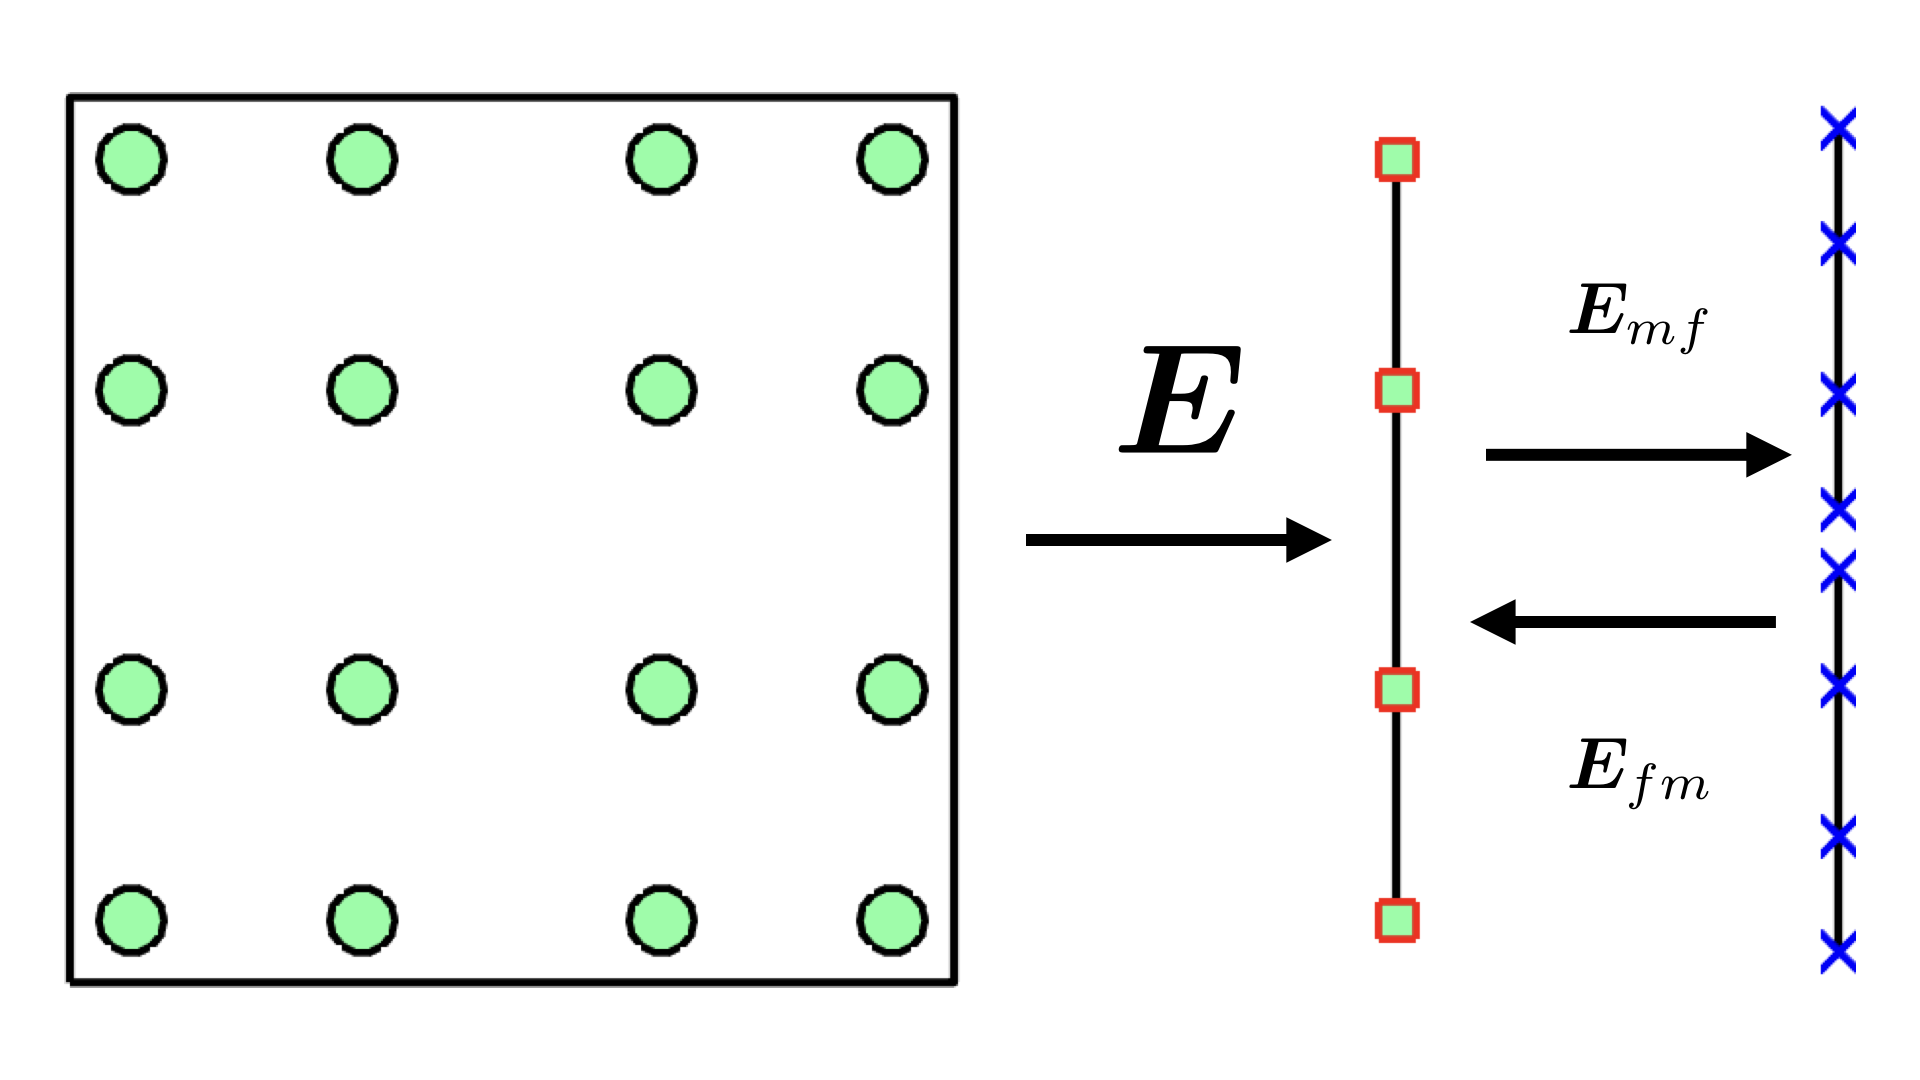
\includegraphics[width=.65\textwidth]{figs/mortar.png}
\caption{Illustration of mortar operators.  The matrix $\bm{E}$ maps from volume quadrature points to surface quadrature points, $\bm{E}_m$ maps from surface to mortar surface points, and $\tilde{\bm{E}}_m$ maps from mortar surface points to surface points. }
\label{fig:gqcon_noncon}
\end{figure}

Let $\bm{V}_q$ and $\bm{V}_f$ denote interpolation matrices which evaluate at volume and surface quadrature points, respectively, and let $\bm{W}, \bm{W}_f$ denote diagonal matrices whose entries consist of volume and surface quadrature weights
\[
\text{\note{add defs of matrices}}
\]

Let $\bm{E} = \bm{V}_f\bm{P}_q$ denote the polynomial mapping which extrapolates values from volume quadrature points to values at surface quadrature points.  We also define $\bm{B}_i$ as the diagonal matrix containing products of quadrature weights and the $i$th component of the outward normal vector $\hat{\bm{n}}_i$
\[
\bm{B}_i = \bm{W}_f \diag{\hat{\bm{n}}_i}.
\]

An entropy stable skew-symmetric formulation can be given on the reference element $\hat{D}$ as follows:
\[
\bm{M}\td{\bm{u}_N}{t} + \begin{bmatrix} \bm{V}_q \\ \bm{V}_f \end{bmatrix}^T
\LRp{\begin{bmatrix}
\bm{Q}_i-\bm{Q}_i^T & \bm{E}^T\bm{B}_i\\
-\bm{B}_i\bm{E} & \bm{0}
\end{bmatrix} \circ \bm{F}_S}\bm{1} + \bm{V}_f^T\bm{B}_i\bm{f}_i^* = 0.  
\]

We incorporate mortars by modifying this formulation.  Let $\bm{V}_m$ denote the matrix which maps volume quadrature points to values at surface \textit{mortar} points.  We also need to introduce interpolation operators $\bm{T}_f, \bm{T}_m$ for surface trace spaces.  Here, $\bm{T}_f$ maps from polynomials on the surface $\partial \hat{D}$ to surface quadrature points, while $\bm{T}_m$ maps from polynomials on $\partial \hat{D}$ to mortar quadrature points.  We can then define surface and mortar mass and projection matrices
\begin{align*}
\bm{M}_m = \bm{T}_m^T\bm{W}_m\bm{T}_m, \qquad \bm{P}_m = \bm{M}_m^{-1}\bm{T}_m^T\bm{W}_m\\
\bm{M}_f = \bm{T}_f^T\bm{W}_f\bm{T}_f, \qquad \bm{P}_f = \bm{M}_m^{-1}\bm{T}_f^T\bm{W}_f.
\end{align*}
Note that we have used the mortar mass matrix $\bm{M}_m$ in the above definition of the face projection.  This is only necessary if the surface and mortar quadratures do not exactly integrate degree $2N$ polynomials.  If both the surface and mortar quadratures are exact for polynomials of degree $2N$, then $\bm{M}_m = \bm{M}_f$, and no distinction is necessary between the two mass matrices.  

\begin{remark}
In order to show stability, we require that both $\bm{P}_f$ and $\bm{P}_m$ are defined using the same mass matrix.  We have used the mortar mass matrix $\bm{M}_m$ here; however, we could also use the surface mass matrix $\bm{M}_f$ in both $\bm{P}_f$ and $\bm{P}_m$.  We use the mortar mass matrix in this work, as the mortar quadrature is generally more accurate than the surface quadrature for our use cases (e.g.\ hybrid and non-conforming meshes).  
\end{remark}


We can now define operators which map between surface and mortar quadrature points.  Let $\bm{E}_m$ denote the map from surface to mortar points, and let $\tilde{\bm{E}}_m $ denote the map from mortar to surface points.  Both operators are defined through an $L^2$ projection to the trace space and interpolation to appropriate points
\[
\bm{E}_m = \bm{T}_m \bm{P}_f, \qquad \tilde{\bm{E}}_m = \bm{T}_f \bm{P}_m.
\]  
We also define a mortar boundary matrix
\[
\tilde{\bm{B}}_i = \bm{W}_m\diag{\hat{\bm{n}}_i}.
\]
Then, a mortar-based formulation can be given as follows:
\begin{equation}
\bm{M}\td{\bm{u}_N}{t} + \begin{bmatrix} \bm{V}_q \\ \bm{V}_f \\ \bm{V}_m \end{bmatrix}^T
\LRp{\begin{bmatrix}
\bm{Q}_i-\bm{Q}_i^T & \bm{E}^T\bm{B}_i &\\
-\bm{B}_i\bm{E} &  & \bm{B}_i\tilde{\bm{E}}_m \\
& -\tilde{\bm{B}}_i{\bm{E}}_m & 
\end{bmatrix} \circ \bm{F}_S}\bm{1} + \bm{V}_m^T\tilde{\bm{B}}_i\bm{f}_i^* = 0.  
\label{eq:mortar}
\end{equation}
Here, we have appended an extra row and column to the decoupled SBP matrix, and the inter-element numerical flux $\bm{f}^*$ is now computed in terms of the \emph{mortar} nodes.  

We first note that
\begin{align*}
\bm{B}_i\tilde{\bm{E}}_m &= \diag{\bm{W}_f} \bm{T}_f \bm{P}_m = \diag{\hat{\bm{n}}} \bm{W}_f \bm{T}_f \bm{M}_m^{-1}\bm{T}_m\bm{W}_m\\
&=  \bm{W}_f \bm{T}_f \bm{M}_m^{-1}\bm{T}^T_m\bm{W}_m\diag{\hat{\bm{n}}_i} = \bm{P}_f^T\bm{T}^T_m \tilde{\bm{B}}_i = \LRp{\tilde{\bm{B}}_i{\bm{E}}_m}^T
\end{align*}
where we have used that $\bm{W}_m$ is diagonal and that the outward normal $\hat{\bm{n}}_i$ on the reference element is constant over each face.  This implies skew-symmetry of the decoupled SBP operator and entropy stability of the overall system.    


\note{Finish}

\section{A mortar-based implementation}

While the formulation presented above is convenient for analysis, it is computationally expensive to implement.  However, using properties of the mortar matrices $\bm{E}_m, \tilde{\bm{E}}_m$, we can rewrite the above formulation in a way which reflects a traditional mortar-based finite element implementation.  In other words, we wish to implement (\ref{eq:mortar}) such that the only modification from the implementations in \cite{chan2017discretely} is a pre-processing step on mortar faces.  

We first note that, since $\bm{E}_m$ maps from surface nodes to mortar nodes, $\bm{V}_m = \bm{E}_m \bm{V}_f$.  Thus, we can rewrite the numerical flux contribution as
\begin{align*}
 \bm{V}_m^T\tilde{\bm{B}}_i\bm{f}_i^* &= \bm{V}_f^T \bm{E}_m^T \bm{W}_m\diag{\hat{\bm{n}}_i} \bm{f}_i^* = \bm{V}_f^T  \bm{P}_f^T\bm{T}_m^T\bm{W}_m\diag{\hat{\bm{n}}_i} \bm{f}_i^*\\
 &= \bm{V}_f^T \bm{W}_f \diag{\hat{\bm{n}}_i} \bm{T}_m\bm{M}_m^{-1}\bm{T}_m^T\bm{W}_m \bm{f}_i^* =  \bm{V}_f^T \bm{B}_i \tilde{\bm{E}}_m\bm{f}_i^*.
\end{align*}

We can similarly reformulate the remaining mortar contributions within (\ref{eq:mortar}).  We decompose $\bm{F}_S$ into interactions between volume nodes, surface nodes, and mortar nodes
\[
\bm{F}_S = \begin{bmatrix}
\bm{F}_S^{vv} & \bm{F}_S^{vs} & \bm{F}_S^{vm}\\
\bm{F}_S^{sv} & \bm{F}_S^{ss} & \bm{F}_S^{sm}\\
\bm{F}_S^{mv} & \bm{F}_S^{ms} & \bm{F}_S^{mm}
\end{bmatrix}
\]
Then, the on-element contributions to (\ref{eq:mortar}) can be expanded as follows
\begin{align*}
&\begin{bmatrix} \bm{V}_q \\ \bm{V}_f \\ \bm{V}_m \end{bmatrix}^T
\LRp{\begin{bmatrix}
\bm{Q}_i-\bm{Q}_i^T & \bm{E}^T\bm{B}_i &\\
-\bm{B}_i\bm{E} &  & \bm{B}_i\tilde{\bm{E}}_m \\
& -\tilde{\bm{B}}_i{\bm{E}}_m & 
\end{bmatrix} \circ \bm{F}_S}\bm{1} \\
&= 
\begin{bmatrix} \bm{V}_q \\ \bm{V}_f \end{bmatrix}^T
\LRp{\begin{bmatrix}
\bm{Q}_i-\bm{Q}_i^T & \bm{E}^T\bm{B}_i\\
-\bm{B}_i\bm{E} & \\
\end{bmatrix} \circ \bm{F}_S}\bm{1} \\
&+ \bm{V}_f^T \LRp{\bm{B}_i\tilde{\bm{E}}_m\circ \bm{F}_S^{sm}}\bm{1} - \bm{V}_m^T \LRp{ \tilde{\bm{B}}_i\bm{E}_m \circ \bm{F}_S^{ms}}\bm{1}
\end{align*}
Since multiplication by diagonal matrices $\bm{B}_i, \tilde{\bm{B}}_i$ is associative under the Hadamard product, the latter terms can be rewritten as 
\begin{align*}
 \bm{V}_f^T \LRp{\bm{B}_i\tilde{\bm{E}}_m\circ \bm{F}_S^{sm}}\bm{1} &=  \bm{V}_f^T \bm{B}_i \LRp{\tilde{\bm{E}}_m\circ \bm{F}_S^{sm}}\bm{1}\\
\bm{V}_m^T \LRp{ \tilde{\bm{B}}_i\bm{E}_m \circ \bm{F}_S^{ms}}\bm{1} &= \bm{V}_m^T \tilde{\bm{B}}_i \LRp{ \bm{E}_m \circ \bm{F}_S^{ms}}\bm{1} = \bm{V}_f^T \bm{B}_i \tilde{\bm{E}}_m \LRp{ \bm{E}_m \circ \bm{F}_S^{ms}}\bm{1} 
\end{align*}
Then, (\ref{eq:mortar}) can be rewritten as 
\begin{align}
\bm{M}\td{\bm{u}_N}{t} &+ 
\begin{bmatrix} \bm{V}_q \\ \bm{V}_f \end{bmatrix}^T
\LRp{\begin{bmatrix}
\bm{Q}_i-\bm{Q}_i^T & \bm{E}^T\bm{B}_i\\
-\bm{B}_i\bm{E} & \\
\end{bmatrix} \circ \bm{F}_S}\bm{1} + \bm{V}_f^T\bm{B}_i \tilde{\bm{f}}^*_i = 0 \label{eq:mortar2}\\
\tilde{\bm{f}}^*_i &= \tilde{\bm{E}}_m\bm{f}^*_i + \LRp{\tilde{\bm{E}}_m\circ \bm{F}_S^{sm}}\bm{1} - \tilde{\bm{E}}_m \LRp{ \bm{E}_m \circ \bm{F}_S^{ms}}\bm{1} 
\nonumber
\end{align}
If the surface and mortar nodes are identical, then $\bm{E}_m = \tilde{\bm{E}}_m = \bm{I}$ and $\LRp{\tilde{\bm{E}}_m \circ \bm{F}_S^{sm}}\bm{1} = \LRp{ \bm{E}_m \circ \bm{F}_S^{ms}}\bm{1}$.  The correction terms within $\tilde{\bm{f}}^*$ cancel out, and we recover the original scheme from \cite{chan2017discretely}.

Note that in (\ref{eq:mortar2}), the only interactions between surface and mortar nodes occurs within the computation of $\tilde{\bm{f}}^*_i$, which can be done solely on mortar interfaces.  The computational structure of 
\begin{enumerate}
\item Compute volume contributions to the RHS
\item Communicate surface contributions to mortar interfaces and compute $\tilde{\bm{f}}^*_i$.
\item Communicate $\tilde{\bm{f}}^*_i$ back to each element.  
\end{enumerate}
%\bm{M}\td{\bm{u}_N}{t} + \begin{bmatrix} \bm{V}_q \\ \bm{V}_f \\ \bm{V}_m \end{bmatrix}^T
%\LRp{\begin{bmatrix}
%\bm{Q}_i-\bm{Q}_i^T & \bm{E}^T\bm{B}_i &\\
%-\bm{B}_i\bm{E} &  & \bm{B}_i\tilde{\bm{E}}_m \\
%& -\tilde{\bm{B}}_i{\bm{E}}_m & 
%\end{bmatrix} \circ \bm{F}_S}\bm{1} + \bm{V}_m^T\tilde{\bm{B}}_i\bm{f}_i^* = 0.  

%It is possible to efficiently interpolate from volume Gauss nodes to split-side Gauss nodes in two steps.  We first interpolate to full-side Gauss nodes on the face, then interpolate from full-side  to split-side Gauss nodes.  Each of these two operations can be done using only one-dimensional interpolation matrices, implying that the interpolation matrix from volume to split-side Gauss nodes can be decomposed into 
%\[
%\bm{V}_{\rm vol-to-split} = \bm{V}_{\rm vol-to-full} \bm{V}_{\rm full-to-split}
%\]
%where each of the matrices in the decomposition possess either a sparse or Kronecker product structure.  
%
%ESDG schemes based on decoupled SBP operators introduced in \cite{chan2017discretely} assume a single interpolation matrix which extrapolates from volume to surface nodes.  These schemes require dyadic flux evaluations between all volume and surface nodes connected by this interpolation matrix.  For non-conforming interfaces with split-side Gauss nodes on the face, this necessitates dyadic flux computations between all volume nodes and all split-side Gauss nodes.  
%
%We show in this section how to construct an entropy stable Gauss collocation scheme based on two layers of surface nodes: full-side and split-side nodes.  These surface nodes will be loosely through a skew-symmetric coupling term involving polynomial interpolation matrices between full-side and split-side nodes.  This scheme requires dyadic flux computations between volume and full-side surface nodes, and between full-side and split-side surface nodes.  Each set of dyadic flux computations can be reduced to 



%We first introduce notation which is helpful for operations involving surface traces.  Let the matrix $\bm{R}$ denote the matrix which maps coefficients of a function to coefficients of its trace.  
%
%Let ${\bm{V}_f}\tilde{P}_f$ denote the matrix which projects to the trace space using split-side quadrature and evaluates at full-side quadrature points.  Similarly, let $\tilde{\bm{V}_f}{P}_f$ denote the matrix which projects to the trace space using full-side quadrature and evaluates at split-side quadrature points
%\begin{align*}
%\bm{C}^i_f &= \begin{pmatrix}
%\bm{0} & {\rm diag}\LRp{\hat{\bm{n}}_i}{\bm{V}_f}\tilde{\bm{P}}_f\\
%-\tilde{\bm{V}_f}{\bm{P}}_f{\rm diag}\LRp{\hat{\bm{n}}_i} &\bm{0}
%\end{pmatrix}, \\
%\bm{S}^i_f &= \begin{pmatrix}
%\diag{\bm{w}_f} & \\
%& \diag{\tilde{\bm{w}}_f}
%\end{pmatrix}\bm{C}^i_f.
%\end{align*}
%It is straightforward to show that the matrix $\bm{S}_f$ is skew-symmetric.
%
%%{fig:gqcon_noncon}
%Let $\tilde{\bm{F}}_S$ denote the flux matrix, then 
%\[
%\begin{bmatrix}\bm{L}_f & \tilde{\bm{L}}_f\end{bmatrix} \LRp{\bm{C}^i_f\circ\tilde{\bm{F}}_S}\bm{1}
%\]
%is a skew-symmetric correction term which ensures entropy stability and high order accuracy (through consistency up to quadrature order).   
%
%Since the difference is high order accurate, you can remove this correction term and still get high order accuracy.  However, the spatial entropy RHS is no longer zero if you use inconsistent surface and coupling quadrature without the correction term (\note{prove this}). 
%
%\note{Do we need 3 layers of surface nodes in 3D?  Interpolation to isotropic split-side nodes is a Kronecker product - does that reduce things down?  }

\section{Error estimates}

\note{Weak derivative vs strong derivative error estimates.  SBP yields that the skew-symmetric form is equivalent to weak form.}

\note{Line DG approach can work, but it's flipped: we increase quadrature strength in the direction \emph{orthogonal} to derivative instead.  May improve accuracy over GLL by giving equivalence w/skew form.}

\section{Numerical experiments}

\subsection{Gauss Lobatto quadrature}

\subsection{Gauss quadrature}

\bibliographystyle{unsrt}
\bibliography{dg}


\end{document}


